\documentclass{beamer}
\usepackage[polish]{babel}
\usepackage[utf8]{inputenc}
\usepackage{lmodern}
\usetheme{AGH}

\title{Zrównoleglenie algorytmu gradientowej klasteryzacji z użyciem technologii GPU}
\subtitle{Ernest Jęczmionek}
\author{dr hab. inż. Piotr Kowalski}
\institute{Wydział Fizyki i Informatyki Stosowanej}
\date{\today}


\begin{document}

\titleframe[pl]

\begin{frame}\frametitle{Plan prezentacji} %\framesubtitle{...z podtytułem...}
	\tableofcontents
\end{frame}

\section{Algorytm klasteryzacji gradientowej}
\begin{frame}\frametitle{Schemat algorytmu klasteryzacji gradientowej}
\begin{enumerate}
	\item sformułowanie estymatora jądrowego wraz z jego parametrami
	\item wykonanie przemieszczeń aż do spełnienia warunku zakończenia
	\item procedura tworzenia klastrów
\end{enumerate}
\end{frame}

\begin{frame}\frametitle{Estymator jądrowy}
\begin{center}
$\hat{f}(x)=\frac{1}{mh^n} \displaystyle \sum_{i=1}^{m} \frac{1}{s_i}K(\frac{x-x_i}{hs_i})$ \\~\
gdzie $h = min(g(h))$ \\~\
$g(h)=\frac{1}{m^2h^2}\displaystyle\sum_{i=1}^{m} \displaystyle\sum_{j=1}^{m} \widetilde{K}(\frac{x_j - x_i}{h}) + \frac{2}{mh^n}K(0)$ \\~\
$s_i = {\frac{\hat{f}_*(x_i)}{\bar{s}}}^{-c}$ \\~\
\end{center}
\end{frame}

\begin{frame}\frametitle{Warunek zakończenia}
\begin{center}
$x_j^{k+1} = x_j^k + b\frac{\nabla f(x_j^k)}{f(x_j^k)}$ \\~\
dopóki $|D_k - D_{k-1}| \leq \alpha D_0$ \\~\
gdzie $D_k = \displaystyle\sum_{i=1}^{m-1} \displaystyle\sum_{j=i+1}^{m} d(x_i^k, x_j^k)$
\end{center}
\end{frame}

\begin{frame}\frametitle{Wyznaczenie odległości międzyklastrowej}
\begin{center}
należy wyznaczyć zbiór wszytkich odległości między elementami \\~\
$\{d(x^{k*}_i, x^{k*}_j)\}$ \\~\
oraz znaleźć najniejszy element zbiotu \\~\
$\{0.01 \sigma_d, 0.02 \sigma_d, ... , int(100D-1) 0.01 \sigma_d \}$ \\~\
spełniający warunek \\~\
$\hat{f}_d(x-0.01\sigma_d) > \hat{f}_d \wedge \hat{f}_d \leq \hat{f}_d(x+0.01\sigma_d)$
\end{center}
\end{frame}

\begin{frame}\frametitle{Procedura tworzenia klastrów}
\begin{enumerate}
\item pobierz element zbioru i utwórz z niego jednoelementowy klaster
\item znajdź inny element w odległości $x_d$ i dodaj go do klastru, gdy jest to niemożliwe przejdź do Punktu 4
\item znajdź inny element w odległości $x_d$ od dowolnego elementu klastru i dodaj go oraz powtórz Punkt 3
\item zaakceptuj utworzony klaster i usuń ze zbioru jego elementy, gdy zbiór nie jest pusty powróć do Punktu 1
\end{enumerate}
\end{frame}


%----------------------------------------------------------


\section{Implementacja}
\begin{frame}\frametitle{Procedura tworzenia klastrów}
\begin{center}
Niniejszy fragment algorytmu jest sekwencyjny!
\end{center}
\end{frame}

%	\footnote{http://home.agh.edu.pl/\~kulpi/publ/Kulczycki\_Charytanowicz\_-\_Applied\_Mathematics\_and\_Computer\_Science\_-\_2010.pdf}



\begin{frame}
\begin{center}
\Huge Dziękuję za uwagę
\end{center}
\end{frame}



%\begin{frame}\frametitle{Dlaczego GPU}
%\begin{figure}
%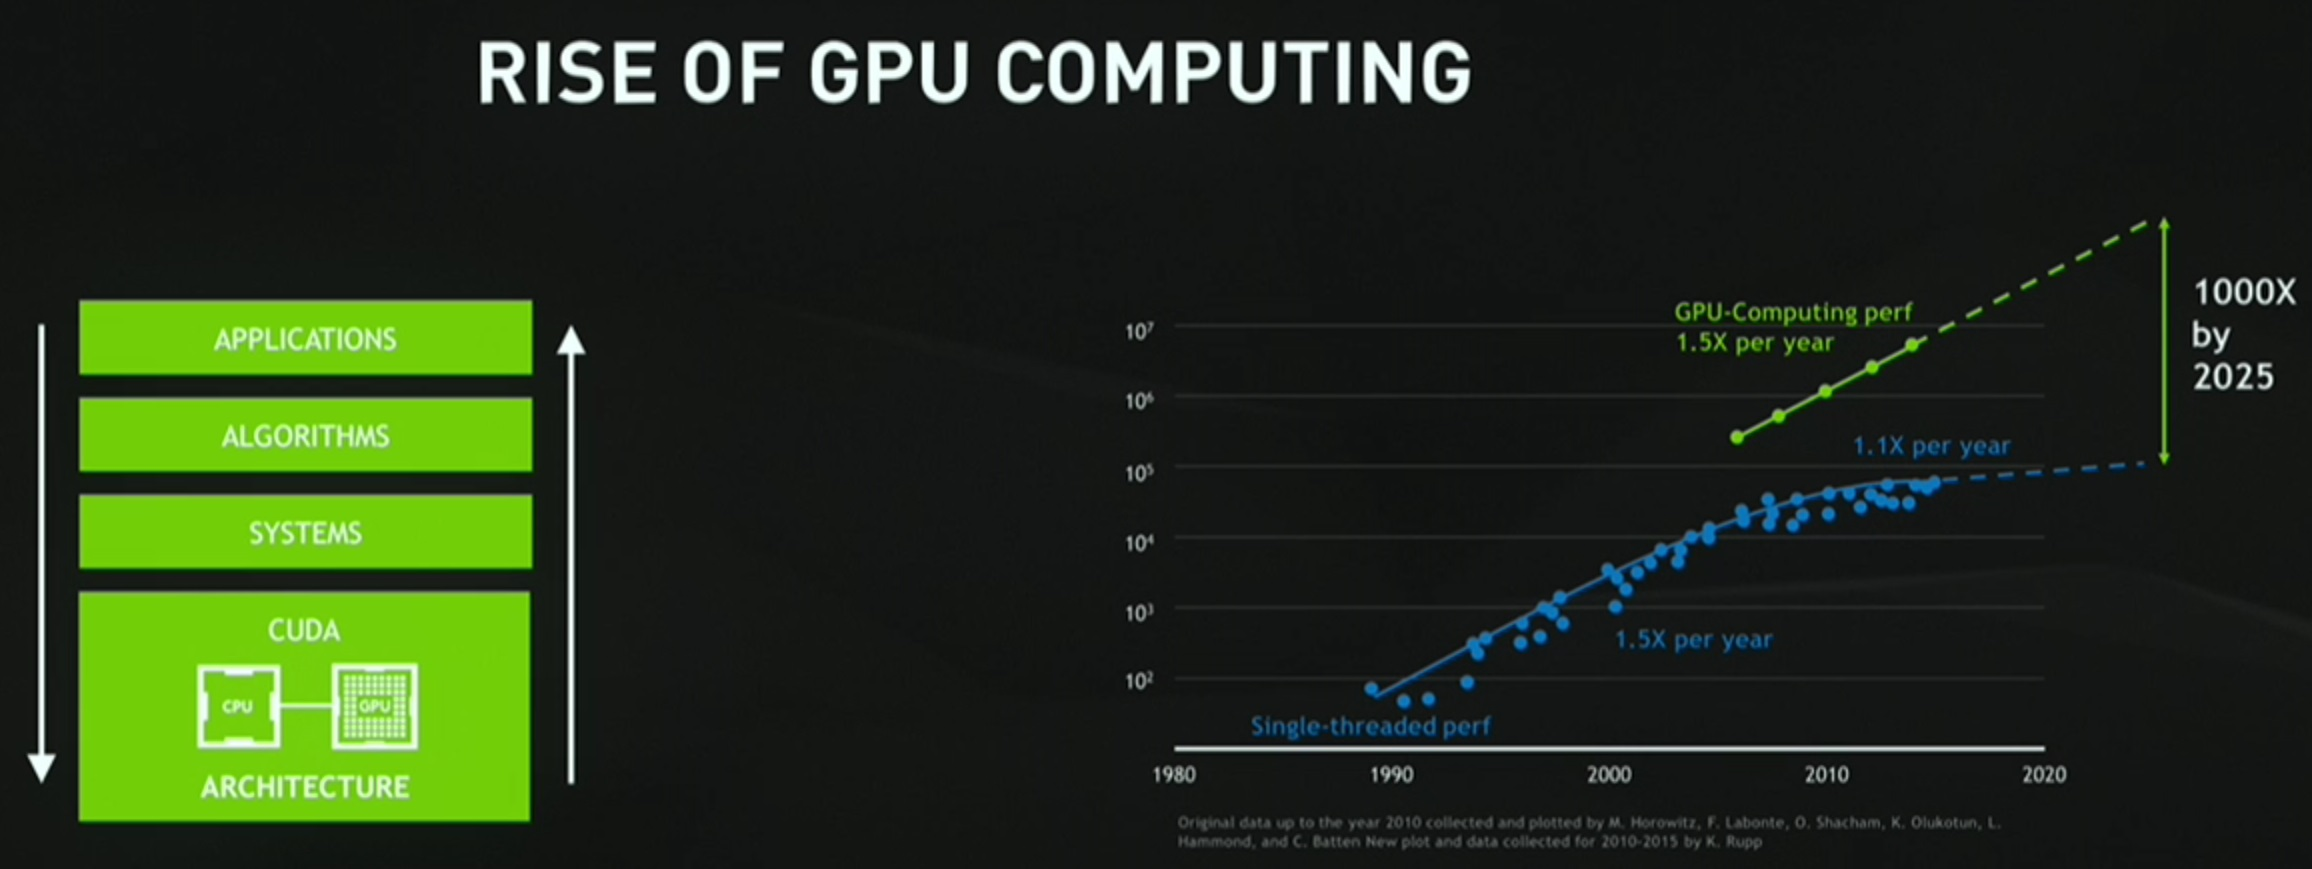
\includegraphics[width=\textwidth]{gpu-performance}
%\end{figure}
%\end{frame}
%
%\section{Wyniki}
%\begin{frame}\frametitle{Frameworki obliczeń równoległych GPGPU}
%\begin{figure}[!htbp]
%	\begin{minipage}[c]{0.48\textwidth}
%	\centering
%	\includegraphics[width=0.48\textwidth]{nvidia}
%	\end{minipage}
%	\begin{minipage}[c]{0.48\textwidth}
%	\centering
%	\includegraphics[width=0.48\textwidth]{OpenCL_Logo}
%	\end{minipage}
%\end{figure}
%\footnote{http://international.download.nvidia.com/partnerforce-us/Brand-Guidelines/NVIDIA\_Logo\_Guidelines\_2012\_1.0.pdf}
%\footnote{https://en.wikipedia.org/wiki/OpenCL\#/media/File:OpenCL\_Logo.svg}
%\end{frame}

\end{document}
